\chapter{Release 3 : Workflow du Budget Non-Industriel (Sprint 4)}
\label{chap:sprint_4}

\section{Introduction}
Les précédents sprints ont permis de maîtriser la capacité de production liée directement au produit automobile (machines de coupe, surface d'assemblage). Toutefois, le bon fonctionnement d'une usine COFAT dépend également d'un écosystème d'investissements dits "non-industriels" : modernisation de l'infrastructure informatique (IT), aménagement des bâtiments (Building), ou achats logistiques. La gestion de ce budget, traditionnellement réalisée par des allers-retours de courriels sans traçabilité, nécessitait une digitalisation urgente. Ce cinquième chapitre, couvrant le Sprint 4 (Release 3), clôture la réalisation technique du projet. Nous commencerons par définir les objectifs et la complexité technique de ce sprint, modélisés à travers le backlog spécifique. Ensuite, nous détaillerons le workflow collaboratif budgétaire implémenté, en insistant sur le rôle volontairement restreint de l'Acheteur (Achat) et l'absence d'étape de validation contraignante par l'Administrateur. Le mécanisme de notifications en temps réel, garantissant la fluidité des échanges, sera expliqué d'un point de vue backend (Node.js) et frontend (React). Enfin, nous présenterons les fonctionnalités d'exportation (Excel/PDF) destinées à la direction, analyserons l'interface utilisateur finalisée, et conclurons sur la robustesse de l'ensemble de l'application \textit{Cofat Capacity Study}.

Ce sprint occupe une place particulière dans la chronologie du projet : contrairement aux sprints précédents qui digitalisaient chacun un processus déjà partiellement outillé (même sommairement, via Excel), le Sprint 4 a nécessité de concevoir de toutes pièces un processus qui n'existait auparavant que sous une forme purement informelle, reposant sur des échanges téléphoniques et des courriels non structurés entre les sites et le département Achats central. Cette absence de processus préexistant à digitaliser a paradoxalement offert une liberté de conception plus grande, mais a également exigé un travail de modélisation métier plus approfondi en amont avec le Product Owner, afin de s'assurer que le workflow proposé corresponde fidèlement aux pratiques réelles du département Achats plutôt qu'à une vision théorique idéalisée du processus.

\section{Objectifs et complexité du Sprint 4}
Le développement d'un workflow financier au sein d'une SPA (Single Page Application) est techniquement plus ardu que la simple manipulation de données. Ce sprint intègre une forte logique d'état asynchrone entre différents profils d'utilisateurs, chacun disposant d'une vue partielle et d'un droit d'action distinct sur une même ressource partagée : la ligne de budget. Contrairement aux sprints précédents où chaque acteur gérait exclusivement ses propres données (le Site Manager sur son site, l'Admin sur son référentiel global), le Sprint 4 introduit pour la première fois une collaboration inter-rôles sur un même enregistrement de la base SQL Server, ce qui impose une rigueur particulière dans la gestion des accès concurrents et dans la conception du modèle de données.

Les objectifs fixés avec le Product Owner étaient les suivants :
\begin{enumerate}
    \item Permettre la création et la soumission de demandes de budget non-industriel structurées par département.
    \item Implémenter un tunnel de modification stricte des prix par le département Achat, avec un recalcul automatique côté serveur.
    \item Assurer une traçabilité des modifications via un système d'alerte (notifications) instantané.
    \item Générer des rapports binaires professionnels téléchargeables (exports).
\end{enumerate}

Chacun de ces quatre objectifs répond à une limite précise identifiée dans l'ancien processus manuel décrit au chapitre 1 : l'absence de structuration des demandes (résolue par l'objectif 1), le manque de contrôle sur qui peut modifier quoi (résolu par l'objectif 2, qui restreint chirurgicalement le rôle Achat à 2 colonnes uniquement : \texttt{unitPrice} et \texttt{currency}), la perte de traçabilité des échanges par courriel (résolue par l'objectif 3), et la difficulté de consolider l'information pour la Direction (résolue par l'objectif 4).

\textbf{Modèles de données impliqués :}
Pour soutenir ces objectifs, deux modèles Sequelize majeurs ont été implémentés dans la base SQL Server :
\begin{itemize}
    \item \textbf{\texttt{NonIndustrialBudget}} : Stocke la demande financière. Ses champs réels sont \texttt{department} (IT, HR, QUALITY, BUILDING, LOGISTICS, MAINTENANCE, PRODUCTION), \texttt{area}, \texttt{equipment}, \texttt{qty}, \texttt{currency}, \texttt{unitPrice}, \texttt{totalPrice} (calculé par hook), \texttt{createdBy}, et \texttt{updatedBy}.
    \item \textbf{\texttt{BudgetNotification}} : Stocke la piste d'audit et les messages. Ses champs sont \texttt{type} (NEW\_REQUEST, PRICE\_UPDATED), \texttt{message}, \texttt{isRead}, \texttt{budgetItemId}, \texttt{fromUser}, \texttt{toRole}, et \texttt{toUser}.
\end{itemize}

Le choix de séparer \texttt{NonIndustrialBudget} et \texttt{BudgetNotification} en deux tables distinctes, plutôt que d'intégrer un simple champ de statut dans la première, répond à un besoin de conception précis : conserver un historique complet et non destructif de toutes les actions effectuées sur une ligne budgétaire. Si l'on avait uniquement stocké le statut courant dans \texttt{NonIndustrialBudget}, toute modification successive du prix par l'Achat aurait écrasé l'information précédente, rendant impossible la reconstitution chronologique des négociations. La table \texttt{BudgetNotification}, par sa relation \texttt{1..N} avec \texttt{NonIndustrialBudget} (une ligne de budget peut accumuler plusieurs notifications au fil du temps), constitue de fait un journal d'audit léger, consultable a posteriori par n'importe quel utilisateur autorisé souhaitant comprendre l'historique d'une demande.

Le champ \texttt{department} de \texttt{NonIndustrialBudget} n'est volontairement pas une simple chaîne de caractères libre côté formulaire React : il est contraint par une liste énumérée correspondant aux grandes directions transverses de COFAT (IT, RH, Qualité, Bâtiment, Logistique, Maintenance, Production). Cette contrainte au niveau du frontend, doublée d'une validation identique côté backend Express avant l'insertion Sequelize, garantit la cohérence des données lors des agrégations statistiques ultérieures (voir Section \ref{sec:export_excel_pdf}), en évitant la dispersion de libellés proches mais orthographiés différemment (par exemple "Informatique" contre "IT").

\section{Backlog du Sprint 4}
Le tableau \ref{tab:backlog_sprint4} récapitule les User Stories développées durant ce mois d'août 2026. La complexité de ce sprint ne résidait pas dans les interfaces graphiques, mais dans la synchronisation de l'état React entre les sessions parallèles du Site Manager et de l'Acheteur, ainsi que dans la génération de fichiers binaires (PDF/XLSX) côté serveur Node.js.

\begin{table}[h]
\centering
\begin{tabular}{|p{2cm}|p{8cm}|p{2cm}|p{2cm}|}
\hline
\textbf{ID US} & \textbf{Description} & \textbf{Acteur} & \textbf{Complexité} \\ \hline
US-11 & En tant que Site Manager, je veux saisir et soumettre des lignes de budget avec recalcul auto du total. & Site Mgr & Moyenne \\ \hline
US-12 & En tant qu'acheteur, je veux modifier les 2 colonnes autorisées (prix unitaire et devise) des demandes soumises. & Achat & Haute \\ \hline
US-13 & En tant qu'utilisateur, je veux voir une cloche de notification se mettre à jour lors d'une action budgétaire. & Tous & Haute \\ \hline
US-14 & En tant qu'admin, je veux exporter le tableau budgétaire au format Excel ou PDF. & Admin & Moyenne \\ \hline
\end{tabular}
\caption{Backlog spécifique du Sprint 4}
\label{tab:backlog_sprint4}
\end{table}

Afin de garantir que chaque User Story soit testable et non ambiguë, nous avons formalisé des critères d'acceptation découlant directement de la description de chaque US :

\begin{itemize}
    \item \textbf{US-11 (Création et soumission)} : le formulaire ne doit pas permettre la soumission si le champ \textit{Quantity} ou \textit{Unit Price} est vide ou négatif ; le champ \textit{Total Price} doit se recalculer instantanément côté client à chaque frappe, avant même la validation serveur, pour un retour visuel immédiat à l'utilisateur ; une ligne nouvellement créée doit apparaître dans la liste des demandes de l'Achat uniquement après le passage explicite au statut "Submitted".
    \item \textbf{US-12 (Modification du prix)} : toute tentative de modification d'un champ autre que \texttt{unitPrice} ou \texttt{currency} par un utilisateur de rôle Achat doit être rejetée par le serveur (HTTP 403), indépendamment de ce que le frontend autorise visuellement ; le \texttt{totalPrice} doit refléter exactement $qty \times unitPrice$ après chaque modification.
    \item \textbf{US-13 (Notifications)} : le compteur de la cloche doit s'incrémenter dans la minute suivant l'action déclenchante, sans nécessiter de rafraîchissement manuel de la page ; le clic sur une notification doit la marquer comme lue de façon persistante en base de données.
    \item \textbf{US-14 (Export)} : le fichier généré doit contenir l'intégralité des lignes visibles à l'écran au moment de la demande d'export, y compris celles affectées par un filtre de département actif.
\end{itemize}

\section{Le Workflow Budgétaire : Scénario et Permissions}
Le processus métier de demande de budget chez COFAT a été modélisé pour être extrêmement agile. Contrairement aux lourds systèmes ERP (comme SAP) où chaque étape nécessite l'approbation hiérarchique d'un administrateur, notre système privilégie l'action directe. \textbf{Il n'y a aucune étape de validation/rejet formelle par l'Administrateur dans ce workflow}. L'Administrateur surveille, mais n'interfère pas.

Ce choix de conception, validé conjointement avec le Product Owner M. BOUCHOUICHA, part d'un constat opérationnel simple : dans l'organisation réelle de COFAT, la négociation tarifaire avec les fournisseurs relève exclusivement de la compétence du département Achat, qui dispose déjà de la légitimité métier nécessaire pour ajuster un prix sans repasser par une hiérarchie supplémentaire. Ajouter une étape de validation par l'Admin aurait, dans les faits, dupliqué un contrôle déjà exercé en amont par le processus d'appel d'offres fournisseurs, tout en ralentissant artificiellement le circuit de traitement des demandes.

\textbf{Le scénario réel se déroule en deux étapes fluides :}

\begin{table}[h]
\centering
\begin{tabular}{|p{2cm}|p{3.5cm}|p{9.5cm}|}
\hline
\textbf{Étape} & \textbf{Acteur actif} & \textbf{Action métier et réaction du système} \\ \hline
\textbf{1. Création} & Site Manager (Demandeur) & Saisie d'une nouvelle ligne de budget via le formulaire de son usine. Il indique le \textit{Department} (ex~: IT), l'\textit{Equipment} (ex~: Serveur Dell), la \textit{Quantity} et son estimation de prix. Dès la validation du formulaire, la ligne est persistée en base SQL Server et un événement \texttt{NEW\_REQUEST} est créé dans la table \texttt{BudgetNotification}, visible immédiatement par le rôle Achat. \\ \hline
\textbf{2. Édition du Prix} & Acheteur (Achat) & L'Achat se connecte et accède à la liste des demandes de budget. S'il a obtenu un devis fournisseur meilleur marché, il \textbf{modifie uniquement le coût unitaire (unit price) et la devise (currency)}. C'est l'unique action que ce rôle peut effectuer sur la demande. \textbf{Le backend recalcule instantanément le \textit{total price}} ($Qty \times UnitPrice$) via le hook Sequelize \texttt{beforeUpdate}. \\ \hline
\end{tabular}
\caption{Déroulement du workflow du budget non-industriel}
\label{tab:workflow_budget}
\end{table}

\textbf{Sécurité de la logique métier côté serveur :}
Dans le code source Express (\texttt{routers/nonIndustrialBudgetRoutes.js}), la restriction du rôle Achat est strictement implémentée lors d'une requête \texttt{PUT /update/:id}. Le rôle est lu depuis l'en-tête HTTP \texttt{x-user-role} de la requête. Si cet en-tête contient \texttt{'Achat'}, l'algorithme ignore toute tentative de modification de la quantité ou de la description de l'équipement, et n'autorise l'enregistrement que des champs \texttt{currency} et \texttt{unitPrice}.

Cette vérification n'est jamais déléguée au seul frontend. Bien que l'interface React masque déjà visuellement les champs non éditables pour l'Achat (ergonomie), un utilisateur malveillant pourrait techniquement forger une requête HTTP directe (via un outil comme Postman) en tentant de modifier le champ \texttt{qty} ou \texttt{equipment}. C'est pourquoi le middleware d'autorisation, exécuté avant le contrôleur métier, filtre explicitement le corps de la requête (\texttt{req.body}) côté serveur : seuls les champs whitelistés pour le rôle courant sont extraits et transmis à la fonction \texttt{update} de Sequelize, tous les autres champs présents dans la requête étant silencieusement ignorés. Ce principe de sécurité, connu sous le nom de validation côté serveur (\textit{server-side validation}), constitue une défense en profondeur indispensable dans toute application manipulant des données financières sensibles.

De la même manière, le middleware vérifie que l'utilisateur authentifié possède bien le rôle requis (\texttt{Site Manager}, \texttt{Achat}, ou \texttt{Admin} selon la route) avant même d'atteindre le contrôleur, renvoyant un code HTTP 401 (non authentifié) si le cookie JWT est absent ou invalide, et un code HTTP 403 (accès refusé) si l'utilisateur est authentifié mais ne possède pas le rôle nécessaire pour l'action demandée.

\subsection{Diagramme de séquence du workflow}
Pour mieux visualiser l'enchaînement temporel des échanges entre le frontend React, l'API Express et la base de données lors du cas d'usage central de ce sprint (la modification du prix par l'Achat), la Figure \ref{fig:seq_budget} détaille les interactions techniques depuis la création de la ligne de budget jusqu'à la notification finale du Site Manager.

\vspace{0.5cm}
\begin{figure}[H]
    \centering
    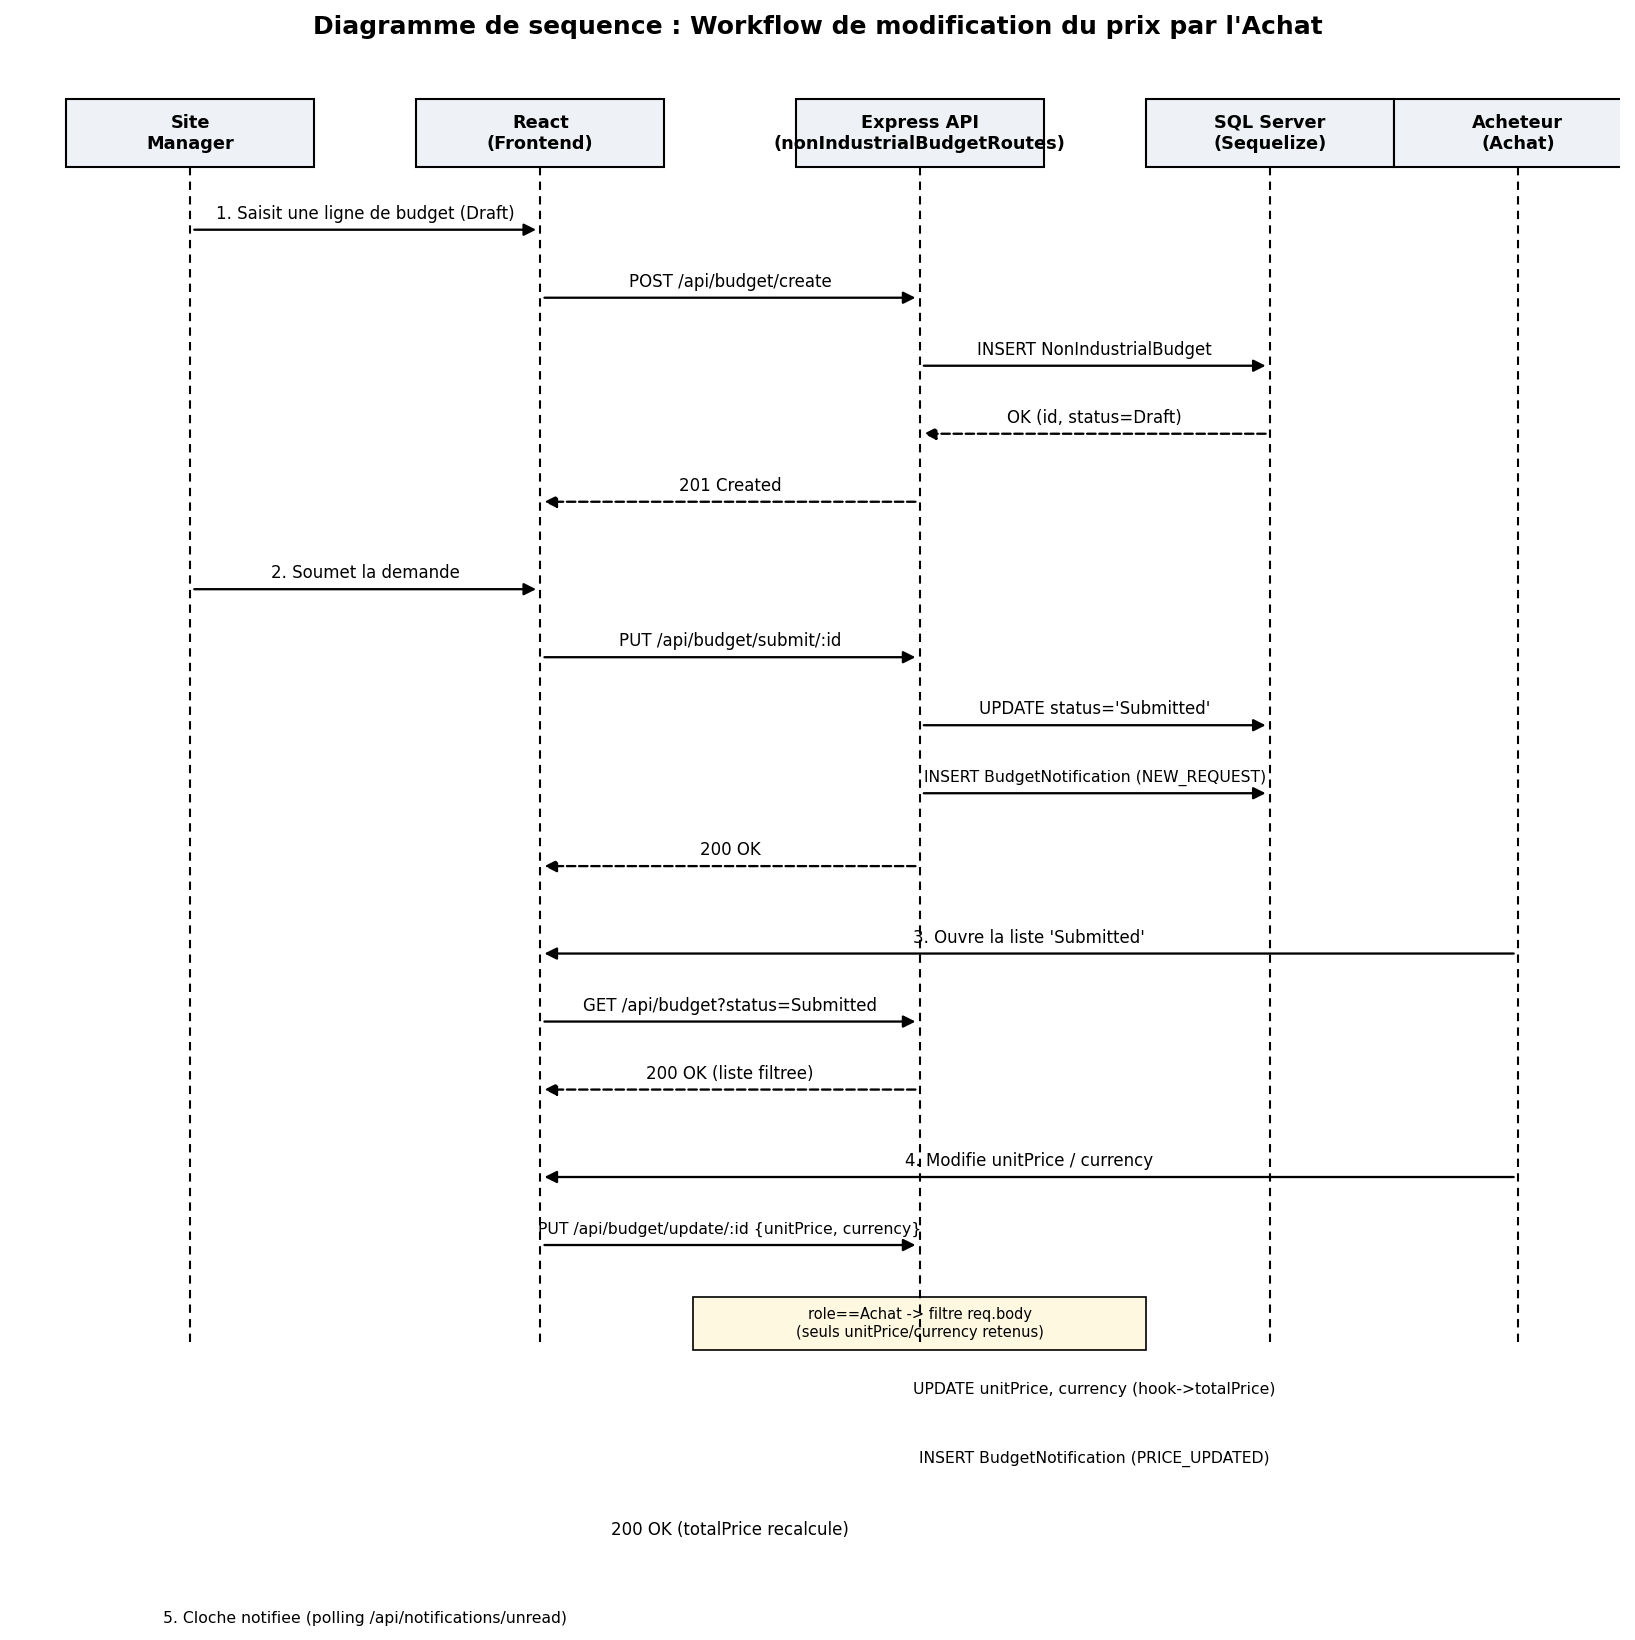
\includegraphics[width=1\textwidth]{img/seq_budget_workflow.png}
    \caption{Diagramme de séquence du workflow de modification du prix par l'Achat}
    \label{fig:seq_budget}
\end{figure}
\vspace{0.5cm}

\textbf{Lecture du diagramme (Figure \ref{fig:seq_budget}) :} les cinq étapes numérotées correspondent exactement au scénario métier décrit dans le Tableau \ref{tab:workflow_budget}, mais font apparaître le détail technique sous-jacent. On y observe notamment que la vérification du rôle Achat (étape encadrée en jaune) s'exécute strictement à l'intérieur du contrôleur Express, avant toute écriture en base — ce qui confirme visuellement qu'aucune requête HTTP, même correctement authentifiée, ne peut contourner la restriction de champs imposée au rôle Achat. On y observe également que la notification (\texttt{INSERT BudgetNotification}) est écrite dans la même transaction logique que la mise à jour du prix, garantissant qu'aucune modification de budget ne puisse avoir lieu sans que la partie prenante concernée ne soit informée, même en cas de défaillance partielle ultérieure du système de polling côté client.

\subsection{Difficultés techniques rencontrées et solutions apportées}
La réalisation de ce sprint a soulevé plusieurs difficultés d'ingénierie qu'il convient de détailler, tant elles ont influencé les choix d'implémentation finaux :

\begin{itemize}
    \item \textbf{Synchronisation de l'état entre sessions concurrentes.} Le Site Manager et l'Achat peuvent être connectés simultanément et consulter la même ligne de budget. Sans mécanisme de rafraîchissement, un Achat pourrait modifier un prix alors que le Site Manager visualise encore une version obsolète de la même ligne. Nous avons résolu ce problème en couplant le \textit{polling} déjà mis en place pour les notifications (Section \ref{sec:notifications_temps_reel}) à un rafraîchissement conditionnel de la grille React : lorsqu'une nouvelle notification de type \texttt{PRICE\_UPDATED} concernant une ligne actuellement affichée est détectée, le composant déclenche automatiquement un nouvel appel \texttt{GET} pour cette ligne spécifique, sans nécessiter de rechargement complet de la page.
    \item \textbf{Prévention des doubles soumissions.} Lors des tests manuels du formulaire d'ajout \textit{inline}, plusieurs clics rapprochés sur le bouton \textbf{ADD NEW ITEM} pouvaient engendrer la création de plusieurs lignes identiques côté serveur avant que l'interface n'ait eu le temps de désactiver le bouton. La solution retenue combine une désactivation immédiate du bouton côté React dès le premier clic (\textit{debounce} visuel) et une contrainte de cohérence côté serveur.
    \item \textbf{Cohérence du calcul du prix total.} Initialement, le recalcul de \texttt{totalPrice} avait été envisagé côté frontend uniquement (calcul JavaScript à l'affichage). Ce choix s'est révélé risqué : en cas de désynchronisation entre deux requêtes concurrentes, deux utilisateurs pouvaient afficher deux totaux différents pour la même ligne. Le recalcul a donc été déplacé exclusivement côté serveur, via le hook Sequelize \texttt{beforeUpdate}, garantissant une source unique de vérité pour cette valeur financière sensible.
    \item \textbf{Gestion des devises multiples.} Le champ \texttt{currency} (TND, USD, EUR, MXN, BRL) reflète la devise locale utilisée par chaque site pour ses négociations non-industrielles. Le système ne procède à aucune conversion automatique entre devises au niveau de la ligne de budget elle-même — chaque ligne conserve sa devise d'origine telle que saisie par le Site Manager ou ajustée par l'Achat, et c'est uniquement au niveau du tableau de bord analytique (Figure \ref{fig:analyse_budget}) que la ventilation est présentée par devise plutôt que consolidée dans une devise unique, évitant ainsi d'introduire un taux de change implicite qui aurait pu fausser la lecture des montants réels négociés.
\end{itemize}

\section{Système de Notifications Temps Réel}
\label{sec:notifications_temps_reel}
Pour remplacer les échanges d'emails asynchrones et informels, le système intègre un moteur de notification intra-applicatif robuste.

\textbf{Mécanisme technique :}
Le serveur Express possède un module \texttt{budgetNotificationHelper.js}. Chaque fois qu'une action budgétaire est interceptée (par exemple, la route POST de création ou la route PUT de mise à jour des prix), une ligne est insérée dans la table \texttt{BudgetNotification}.
\begin{itemize}
    \item Si l'Achat met à jour un prix, le système crée une notification de type \texttt{PRICE\_UPDATED} avec un message textuel décrivant la baisse ou la hausse tarifaire, dirigée spécifiquement vers le \texttt{Site Manager} qui avait créé la ligne (\texttt{toRole: 'User', toUser: budget.createdBy}).
    \item Si un Site Manager modifie sa demande, l'alerte (\texttt{REQUEST\_MODIFIED}) est envoyée vers le groupe \texttt{toRole: 'Achat'}.
\end{itemize}

Ce mécanisme d'aiguillage par \texttt{toRole} et \texttt{toUser} permet de distinguer deux types de diffusion : une notification ciblée vers un individu précis (l'auteur original de la ligne de budget), et une notification diffusée à l'ensemble d'un groupe fonctionnel (tous les membres du rôle Achat, qui peuvent alors se répartir le traitement des nouvelles demandes soumises sans qu'un individu spécifique soit préalablement désigné).

Côté client React, une icône "Cloche" dans la barre de navigation effectue un \textit{polling} (requêtes GET périodiques vers \texttt{/api/notifications/unread}) pour récupérer le compteur. Ce choix technique du \textit{polling}, plutôt qu'une solution de push en temps réel via WebSocket, a été retenu pour sa simplicité d'implémentation et sa robustesse face aux coupures réseau intermittentes qui peuvent survenir sur certains sites industriels éloignés (Cairo, Durango) où la qualité de connexion internet n'est pas toujours homogène avec celle du siège tunisien. Le composant React encapsule cet appel périodique dans un \texttt{useEffect} avec un intervalle défini, nettoyé automatiquement (\texttt{clearInterval}) lors du démontage du composant pour éviter les fuites mémoire.

Au clic, les messages s'affichent et une requête \texttt{PATCH /api/notifications/read} marque les alertes comme lues dans la base de données. L'interface distingue visuellement les notifications non lues (mise en gras, pastille colorée) des notifications déjà consultées, permettant à l'utilisateur de retrouver facilement l'historique de ses échanges avec le département Achat sans avoir à rouvrir chaque ligne de budget individuellement.

\subsection{Conception du contenu des messages}
Un soin particulier a été apporté à la rédaction des messages générés automatiquement par le système, la qualité perçue d'une notification dépendant autant de sa réactivité technique que de la clarté de son contenu. Plutôt que de générer des messages génériques du type "Une modification a eu lieu sur votre demande", chaque message intègre dynamiquement les informations contextuelles pertinentes extraites de la ligne de budget concernée : le nom de l'équipement, le département demandeur, et, dans le cas d'une notification \texttt{PRICE\_UPDATED}, l'ancien et le nouveau prix unitaire, permettant au Site Manager de mesurer immédiatement l'écart obtenu par la négociation de l'Achat sans avoir à rouvrir la ligne concernée. Cette construction dynamique du message est effectuée côté serveur au moment de l'insertion en base, garantissant que le contenu reste figé et fidèle à l'état des données au moment précis de l'action, même si la ligne de budget venait à être modifiée à nouveau par la suite.

\section{Exportation (Excel et PDF)}
\label{sec:export_excel_pdf}
Lors des réunions du Comité de Direction, le besoin d'extraire la donnée du système pour en faire des présentations est indispensable. L'US-14 permet l'exportation des tableaux.

\textbf{Export Excel côté Serveur :}
Plutôt que de générer le fichier dans le navigateur via React (ce qui peut faire planter le navigateur sur de très grands tableaux), l'export est généré sur le serveur Node.js.
Lorsqu'une requête \texttt{GET /api/budget/export/:department} est reçue :
\begin{enumerate}
    \item Sequelize exécute une requête \texttt{findAll} pour récupérer le budget du département demandé.
    \item La bibliothèque \texttt{xlsx} crée un nouveau classeur (\textit{workbook}) en mémoire RAM.
    \item Une feuille (\textit{worksheet}) est ajoutée, contenant les colonnes exactes : \textbf{N°, Department, Area, Equipment, QTY, Currency, Unit Price, Total Price, Status}.
    \item Le fichier est streamé sous forme de buffer binaire (\texttt{Blob}) au navigateur avec l'en-tête HTTP \texttt{Content-Disposition: attachment}, déclenchant le téléchargement du fichier \texttt{.xlsx}.
\end{enumerate}

Ce choix architectural de générer le fichier côté serveur plutôt que côté client présente un avantage supplémentaire non négligeable : il garantit que la donnée exportée provient directement de la source de vérité (la base SQL Server), sans dépendre de l'état potentiellement obsolète du cache React côté navigateur si l'utilisateur avait laissé la page ouverte pendant que d'autres acteurs modifiaient les données en parallèle.

\textbf{Export PDF :}
Une logique similaire est appliquée en utilisant des bibliothèques telles que \texttt{jspdf} et \texttt{jspdf-autotable} pour formater la donnée dans un fichier \texttt{.pdf} prêt à l'impression, avec l'en-tête COFAT et un horodatage officiel. Ce format est privilégié par la Direction lors des comités mensuels, car il offre une mise en page figée, non modifiable par le lecteur, contrairement au fichier Excel qui reste éditable et donc davantage destiné à un usage de retraitement interne par les équipes financières.

\textbf{Sécurité de l'export :} conformément au principe de moindre privilège appliqué sur l'ensemble de l'application, la route d'export est protégée par le même middleware d'authentification par rôle que les autres routes sensibles du module budgétaire, garantissant qu'un utilisateur non autorisé ne puisse pas, en devinant simplement l'URL de la route, télécharger des données financières consolidées auxquelles il n'a pas normalement accès depuis l'interface.

\section{Réalisation du Sprint 4 : Analyse de l'interface}
L'aboutissement de cette architecture asynchrone se concrétise dans une interface moderne et hautement réactive, développée en React/MUI/Tailwind.

\vspace{0.5cm}
\begin{figure}[H]
    \centering
    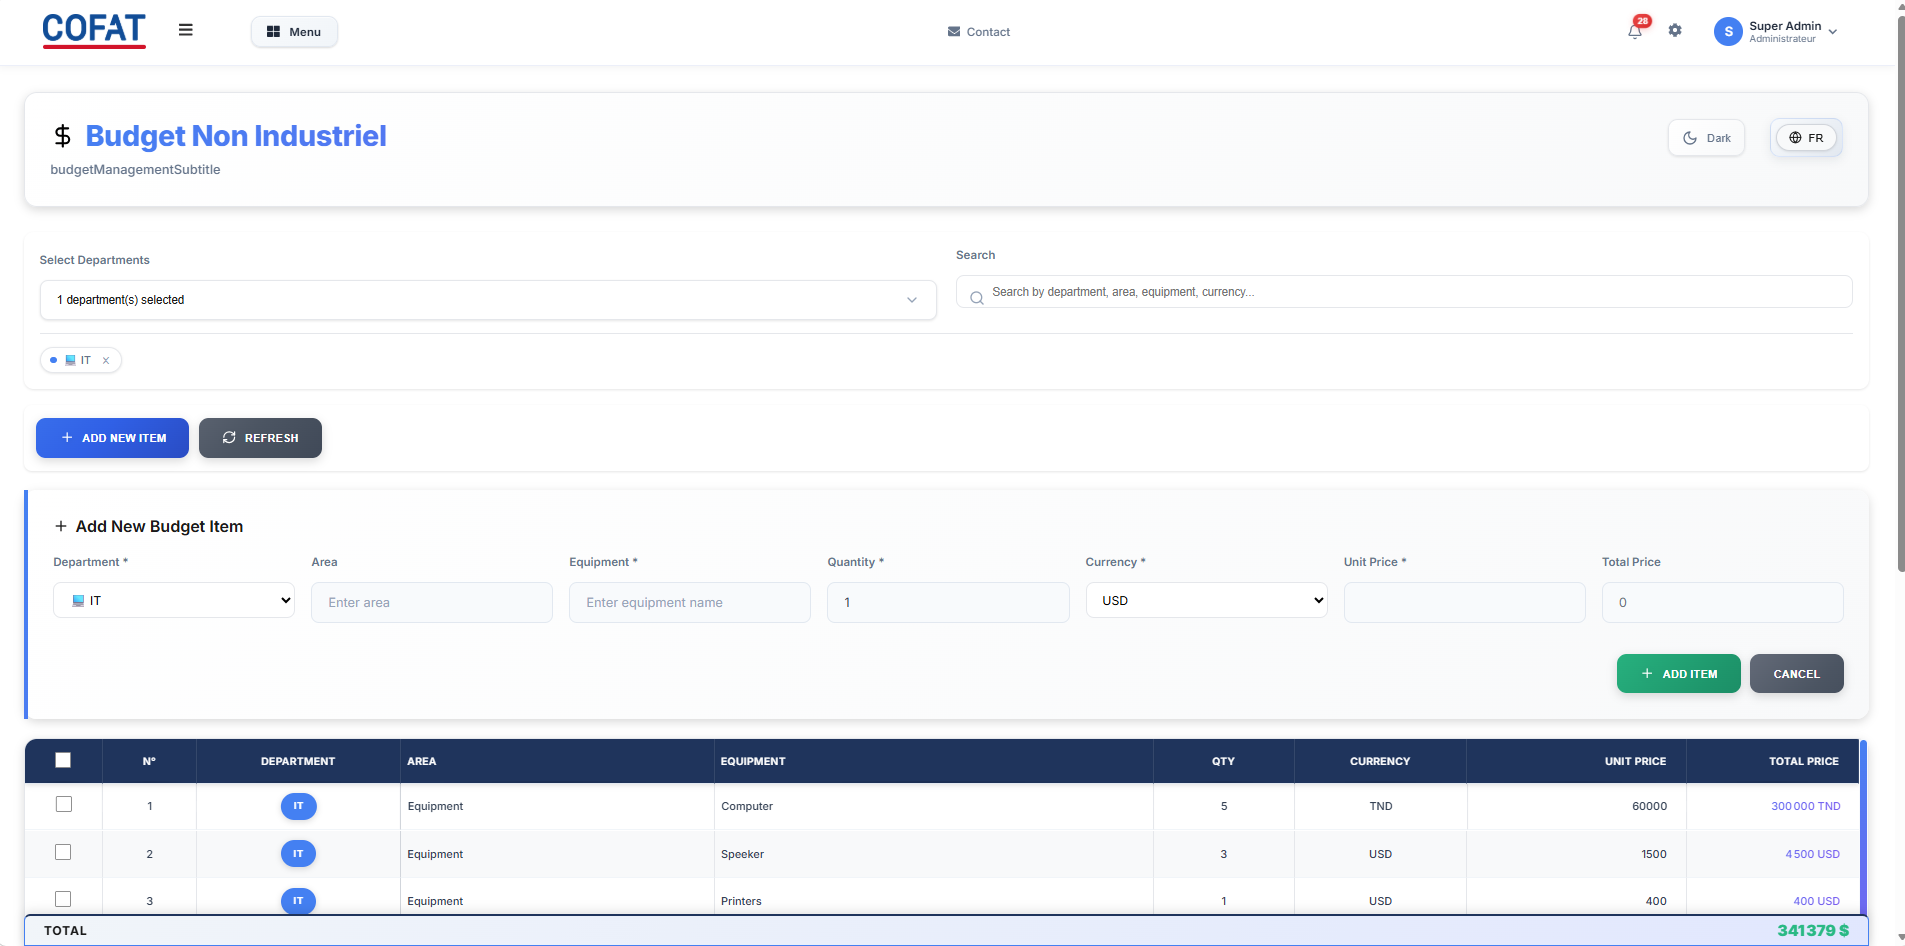
\includegraphics[width=1\textwidth]{img/non industrial budget.png}
    \caption{Interface de gestion dynamique du budget non-industriel}
    \label{fig:non_industrial_budget}
\end{figure}
\vspace{0.5cm}

\textbf{Description de l'interface métier (Figure \ref{fig:non_industrial_budget}) :}
L'écran principal de budgétisation présente un tableau de données exhaustif et dynamique. L'utilisateur y retrouve les colonnes précitées (N°, DEPARTMENT, AREA, EQUIPMENT, QTY, CURRENCY [TND/USD/EUR/MXN/BRL], UNIT PRICE, TOTAL PRICE).
La particularité de cet écran réside dans son formulaire d'ajout \textit{inline} (visible sur la capture), permettant de saisir une nouvelle ligne directement au-dessus du tableau sans ouvrir de fenêtre modale intrusive. Ce choix ergonomique réduit le nombre de clics nécessaires pour un Site Manager qui doit parfois saisir plusieurs dizaines de lignes de budget à la suite lors de la préparation d'un nouveau projet automobile. Des boutons d'action rapides (\textbf{ADD NEW ITEM}, \textbf{REFRESH}) trônent au sommet. Fait notable : le système calcule et maintient en temps réel la \textbf{ligne de TOTAL cumulatif} visible en bas de la grille, adaptant la somme à chaque filtre appliqué ou modification de prix validée par l'Acheteur.

L'interface adapte également dynamiquement les colonnes éditables selon le rôle de l'utilisateur connecté : un Site Manager visualise ses propres lignes en mode saisie complète tant qu'elles sont au statut "Draft", tandis qu'un utilisateur du rôle Achat, en ouvrant la même grille, ne voit que les cellules \textit{Unit Price} et \textit{Currency} devenir interactives (surlignées au survol), toutes les autres colonnes étant affichées en lecture seule. Ce comportement, piloté par une simple condition sur le rôle stocké dans le \textit{Context} d'authentification React, renforce visuellement auprès de l'utilisateur la limite de ses propres permissions, en cohérence avec la restriction déjà imposée côté serveur.

\vspace{0.5cm}
\begin{figure}[H]
    \centering
    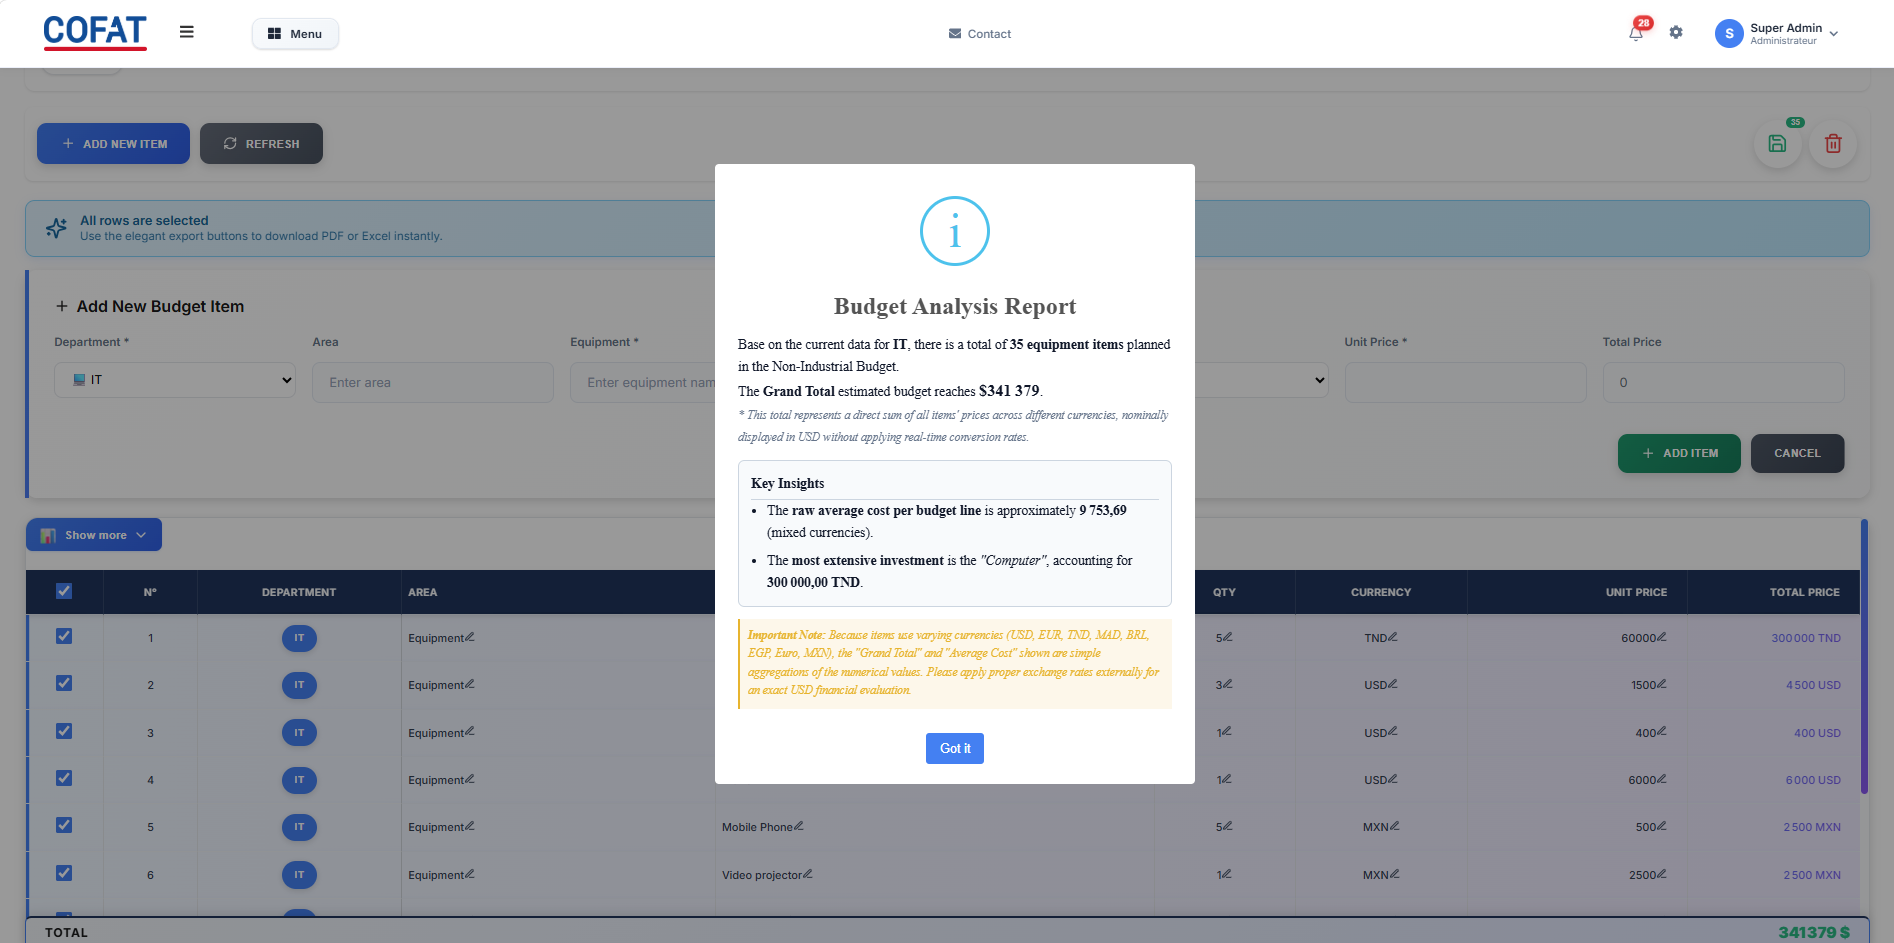
\includegraphics[width=0.9\textwidth]{img/non industrial budget analyse.png}
    \caption{Tableau de bord d'analyse des dépenses par département}
    \label{fig:analyse_budget}
\end{figure}
\vspace{0.5cm}

Afin d'accompagner la validation globale du budget au niveau corporatif, l'interface propose un onglet analytique (Figure \ref{fig:analyse_budget}). Les graphiques (Charts.js) générés par le backend (\texttt{GET /stats/by-department}) ventilent les dépenses non-industrielles par grand département (IT, Qualité, Bâtiment). Le directeur financier de COFAT peut ainsi visualiser immédiatement, via un graphique en anneau (Doughnut chart) et un histogramme par devises, si le budget IT mondial dépasse l'enveloppe allouée pour l'année.

Cette vue analytique répond directement au besoin identifié au chapitre 1 : permettre une prise de décision d'investissement rapide sans attendre la consolidation manuelle habituellement réalisée en fin de trimestre. La ventilation par devise (TND, USD, EUR, MXN, BRL) est particulièrement utile pour le suivi budgétaire consolidé, chaque site historiquement négociant ses achats non-industriels dans la devise locale de son pays d'implantation.

\subsection{Adaptabilité multi-appareils de l'interface budgétaire}
Contrairement aux modules de planification locale du Sprint 2, généralement consultés depuis un poste fixe de bureau par des ingénieurs méthodes, le module de budget non-industriel est fréquemment utilisé par les membres du département Achats en déplacement ou en réunion avec des fournisseurs, souvent depuis une tablette. Cette contrainte d'usage a orienté plusieurs choix ergonomiques : la grille de données bascule automatiquement, sous la largeur d'écran d'une tablette, d'un affichage tabulaire classique vers un affichage en cartes empilées (\textit{cards}) présentant les mêmes informations de façon plus verticale, grâce aux classes utilitaires responsives de Tailwind CSS appliquées sans média-requêtes explicites. Le formulaire de modification du prix unitaire, en particulier, a été spécifiquement testé et ajusté pour rester utilisable au doigt sur un écran tactile, avec des zones de saisie suffisamment grandes pour éviter les erreurs de frappe lors d'une négociation tarifaire réalisée dans l'urgence, en direct au téléphone avec un fournisseur.

\subsection{Synthèse du sprint}
Le tableau \ref{tab:synthese_sprint4} récapitule l'état de clôture des quatre User Stories du Sprint 4 à l'issue de la Sprint Review du 31 août 2026, ainsi que le module technique principal associé à chacune.

\begin{table}[h]
\centering
\begin{tabular}{|p{1.6cm}|p{6.5cm}|p{4cm}|p{2cm}|}
\hline
\textbf{ID US} & \textbf{Module technique principal} & \textbf{Composant clé} & \textbf{Statut} \\ \hline
US-11 & Création/soumission de budget & \texttt{NonIndustrialBudget} + formulaire inline React & Terminée \\ \hline
US-12 & Édition restreinte du prix par l'Achat & Middleware RBAC + hook \texttt{beforeUpdate} & Terminée \\ \hline
US-13 & Notifications temps réel & \texttt{BudgetNotification} + polling React & Terminée \\ \hline
US-14 & Export Excel/PDF & \texttt{xlsx} + \texttt{jspdf-autotable} & Terminée \\ \hline
\end{tabular}
\caption{Synthèse de clôture du Sprint 4}
\label{tab:synthese_sprint4}
\end{table}

Les quatre User Stories ont été livrées et validées lors de la démonstration finale au Product Owner, clôturant ainsi la Release 3 et, par la même occasion, l'ensemble du périmètre fonctionnel initialement défini dans le Backlog Général présenté au chapitre 2.

\subsection{Gestion de l'état applicatif côté React}
Le module de budget non-industriel illustre bien une problématique récurrente du développement d'interfaces riches en React : la gestion cohérente de l'état applicatif à travers plusieurs composants qui doivent réagir aux mêmes événements métier. Trois sources d'état distinctes doivent rester synchronisées à tout instant : la liste des lignes de budget affichées dans la grille MUI, le compteur de notifications non lues affiché dans la cloche de la barre de navigation, et l'éventuel formulaire d'édition ouvert par l'utilisateur.

Plutôt que de recourir à une bibliothèque de gestion d'état globale complexe (comme Redux, jugée disproportionnée pour la taille de l'application), le choix s'est porté sur le \textit{Context API} natif de React déjà utilisé pour la gestion de la session d'authentification depuis le Sprint 1, complété par un système d'événements légers propagés localement entre le composant de notification et le composant de grille budgétaire. Lorsqu'une notification de type \texttt{PRICE\_UPDATED} concernant une ligne actuellement affichée à l'écran est détectée par le polling, un événement personnalisé est déclenché, écouté par le composant de grille, qui rafraîchit alors uniquement la ligne concernée plutôt que l'intégralité du tableau — une optimisation qui évite un effet de clignotement visuel désagréable pour l'utilisateur en cas de mise à jour fréquente.

\section{Conclusion}
Le Sprint 4 a couronné le succès du projet en intégrant la dimension financière à la gestion capacitaire. L'ingénierie mise en place dans le workflow du budget non-industriel prouve la maturité de l'architecture Node.js/React : gestion fine des droits RBAC (restreignant chirurgicalement l'Achat à la modification de 2 colonnes uniquement : \texttt{unitPrice} et \texttt{currency}), recalculs automatiques par l'ORM Sequelize, moteur de notification intra-applicatif et génération de rapports Excel/PDF serveur. Ces fonctionnalités mettent un terme définitif à la perte de traçabilité et aux lourdeurs bureaucratiques des processus antérieurs.

Au-delà de l'aspect purement fonctionnel, ce sprint a également constitué une validation grandeur nature de la robustesse de l'architecture 3-tiers choisie dès le chapitre 3 : la capacité à faire cohabiter, sur une même ressource métier, trois profils d'utilisateurs aux droits strictement différenciés, sans jamais reposer la sécurité sur la seule interface graphique, démontre la maturité technique globale du système. L'application \textit{Cofat Capacity Study} est désormais complète, opérationnelle, et prête à soutenir la stratégie de croissance globale du Groupe COFAT.

En rétrospective sur l'ensemble des quatre sprints réalisés entre mars et août 2026, il apparaît que la contrainte la plus structurante du projet n'a pas été d'ordre purement technique, mais organisationnel : traduire fidèlement, dans le code, des règles de gouvernance et de répartition des responsabilités entre trois métiers aux logiques parfois divergentes (production, direction centrale, achats). Le respect scrupuleux de ce périmètre de permissions, en particulier la restriction volontaire du rôle Achat aux 2 seules colonnes modifiables (\texttt{unitPrice} et \texttt{currency}), toutes les autres colonnes étant verrouillées en lecture seule aussi bien côté frontend qu'au niveau du contrôleur Express, aura été un fil conducteur constant de la phase de réalisation, rappelé et vérifié à chaque sprint plutôt que traité comme un détail d'implémentation secondaire. C'est cette rigueur, autant que la pertinence des choix technologiques eux-mêmes, qui conditionnera la pérennité de l'outil une fois celui-ci pleinement déployé sur l'ensemble des dix sites du groupe.
